% HARM v4: what is new with respect to v3. A technical report (H14).
% Build: make -C doc/report (latexmk -pdf). Checks: doc/report/check.sh, check_coverage.py,
% run_examples.py (ctest -L doc).
\documentclass[11pt,a4paper]{article}

\usepackage[T1]{fontenc}
\usepackage[utf8]{inputenc}
\usepackage{lmodern}
\usepackage{microtype}
\usepackage[margin=2.5cm]{geometry}
\usepackage{amsmath,amssymb}
\usepackage{booktabs}
\usepackage{array}
\usepackage{longtable}
\usepackage{enumitem}
\usepackage{xcolor}
\usepackage{textcomp}
\usepackage{listings}
\usepackage{tikz}
\usetikzlibrary{arrows.meta,positioning,fit,calc,shapes.geometric}
\usepackage[hyphens]{url}
\usepackage[colorlinks=true,linkcolor=blue!50!black,citecolor=green!40!black,urlcolor=blue!50!black]{hyperref}
\usepackage[nameinlink,capitalise]{cleveref}

\newcolumntype{P}[1]{>{\raggedright\arraybackslash}p{#1}}
\setlist{itemsep=2pt,topsep=4pt}
\setlength{\parskip}{3pt}
\setlength{\emergencystretch}{2em}

% ---- code -------------------------------------------------------------------------------------------
\lstdefinestyle{inline}{basicstyle=\ttfamily\small,columns=fullflexible,keepspaces=true,upquote=true}
\lstdefinestyle{block}{basicstyle=\ttfamily\footnotesize,columns=fullflexible,keepspaces=true,
  breaklines=true,upquote=true,frame=single,framesep=4pt,rulecolor=\color{black!30},backgroundcolor=\color{black!3},
  xleftmargin=6pt,xrightmargin=6pt,aboveskip=8pt,belowskip=8pt,showstringspaces=false}
\lstset{style=block}
% \code|...|: inline code (any character but the delimiter)
\newcommand{\code}{\lstinline[style=inline]}
% \opt{reduce}: a command-line option
\newcommand{\opt}[1]{\texttt{-{}-#1}}
% \file{path}: a path in the repository (checked to exist by check_coverage.py)
\newcommand{\file}[1]{\path{#1}}
% decision and milestone references
\newcommand{\dec}[1]{\textsf{#1}}
\newcommand{\ms}[1]{\textsf{#1}}

\title{\textbf{HARM v4}\\[4pt]\large What is new with respect to HARM v3}
\author{Samuele Germiniani\\University of Verona}
\date{Technical report, October 2026}

\begin{document}
\maketitle

\begin{abstract}
HARM is a hint-based miner of temporal assertions from simulation traces. Version~4 is the result of a plan of 28 milestones carried out between v3 and v4. It makes HARM's output deterministic and its SystemVerilog output valid; extends the proposition language with SystemVerilog syntax and documents its semantics on unknown values; adds an option for the end-of-trace semantics of a simulator; removes semantically redundant assertions, proving equivalence of propositions with Z3 and implication between assertions with Spot together with an exact model of HARM's finite-trace evaluation; and lets the RTL guide mining through cones of influence, computed by a new generator, \texttt{harm-coi}, which also harvests the RTL's own predicates. Every new feature is opt-in. This report describes each change, why it was made, the decisions behind it, and how it was validated: every semantic component was checked against an oracle that shares none of its code, and most oracles were themselves checked by planting bugs.
\end{abstract}

\tableofcontents
\newpage

\section{Introduction}\label{sec:intro}

\subsection{HARM v3 in one page}
HARM~\cite{harm-tcad22} mines temporal assertions from the simulation traces of a design. It does not read the design: its inputs are one or more traces (VCD, sampled at the rising edges of a clock, or CSV, one row per cycle) and a configuration of \emph{hints} written by the verification engineer:
\begin{itemize}
\item \textbf{propositions} (\code|<prop exp="cnt == 4'd9"/>|): Boolean expressions over the trace's variables, in C or SystemVerilog syntax;
\item \textbf{numerics} (\code|<numeric>|): arithmetic expressions from which HARM generates propositions by clustering their values~\cite{harm-vlsisoc22};
\item \textbf{templates}: temporal formulas with placeholders, e.g.\ \code!G({..#1&..} |-> P0)! or \code|G(P0 -> X P1)|;
\item \textbf{metrics}: formulas over the features of an assertion (its contingency table \code|atct|, \code|atcf|, \ldots, its complexity, its fault coverage), used to filter and rank.
\end{itemize}
Propositions are grouped into \emph{domains} (\code|loc="a"|, \code|"c"|, \code|"dt"|, or local numbers), which restrict the placeholders they may fill. A \emph{context} groups the hints that are mined together.

Mining runs on three levels of parallelism. For each template (level~3), HARM enumerates the \emph{permutations} that fill its placeholders with propositions of the right domains (level~2). A template may contain one \emph{decision-tree operator} in its antecedent (\code|..&&..|, \code|..##1..|, \code|..#1&..|): for each permutation, a greedy decision tree then grows the antecedent one proposition at a time, keeping the candidates that best separate the cycles where the consequent holds from those where it fails (level~1). Every candidate assertion is evaluated on the traces with a deterministic automaton built by Spot~\cite{spot2}; an assertion is kept if no instance of it fails inside the trace. The kept assertions are qualified: trivial and duplicated ones are removed, metrics filter and rank them, optional edit rules rewrite them, and they are printed in Spot LTL, PSL or SVA.

\subsection{Why v4}
HARM v4 was developed for two uses.
\begin{itemize}
\item \textbf{trivergence}, a project that compares three views of a design: the specification (through an LLM), the RTL, and the simulation traces, with HARM as the trace view. It needed HARM's output to be deterministic, valid SystemVerilog, free of redundant assertions, and able to take structural hints from the RTL. Its adapter worked around several of HARM's limits; v4 removes most of those workarounds.
\item \textbf{Traditional RTL-guided mining}, as GoldMine~\cite{goldmine} does: restricting the search to what the RTL can produce. GoldMine does not support SystemVerilog; v4 can do this for SystemVerilog designs with \texttt{harm-coi}.
\end{itemize}

\subsection{What is new}
\begin{itemize}
\item \textbf{Default output} (\cref{sec:default}): deterministic order; valid SystemVerilog; correct brackets in Spot LTL; SystemVerilog vector indices; bug fixes.
\item \textbf{Proposition language and semantics} (\cref{sec:language}): SystemVerilog literals and operators, invariant templates, skipping invalid propositions, HARM's rule for unknown (\code|x|/\code|z|) values, and the end-of-trace semantics of a simulator as an option.
\item \textbf{Semantic redundancy reduction} (\cref{sec:reduction}): equivalent propositions (Z3), implied assertions (Spot and an exact model of HARM's evaluation), and facts between comparisons.
\item \textbf{Cones of influence} (\cref{sec:coi}): a file format, a rank mode that scores assertions by structural plausibility, a filter mode that prunes the search, with or without depths, and a report of the propositions outside each cone.
\item \textbf{\texttt{harm-coi}} (\cref{sec:harmcoi}): a generator of cones and RTL predicates from SystemVerilog.
\item \textbf{Determinism and portability} (\cref{sec:portability}): one toolchain, Linux and macOS with identical results, the test tools in \file{third_party/}, profiling as an option.
\item \textbf{Validation} (\cref{sec:validation}): the oracles behind each component, and the tests of the oracles.
\end{itemize}
\Cref{sec:limits} lists the known limitations. The appendix is a reference: the new options and XML elements, every decision, and every milestone with its findings.

\Cref{fig:flow} shows how the parts fit. HARM stays independent of the design's source: the RTL is read only by \texttt{harm-coi}, which talks to HARM through a versioned JSON file.

\begin{figure}[t]
\centering
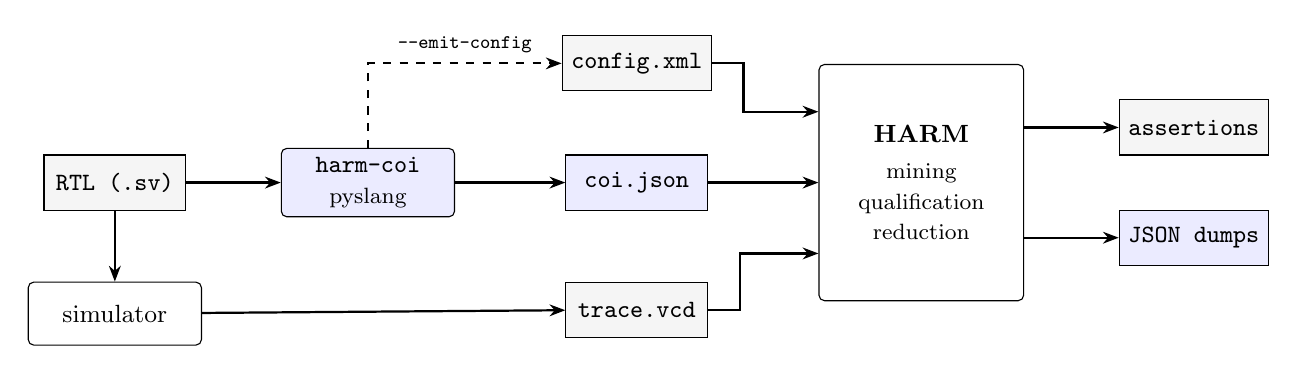
\begin{tikzpicture}[
  box/.style={draw,rounded corners=2pt,minimum height=8mm,minimum width=22mm,align=center,font=\small},
  file/.style={draw,minimum height=7mm,minimum width=18mm,align=center,font=\small\ttfamily,fill=black!4},
  new/.style={fill=blue!8},
  arr/.style={-{Stealth[length=2mm]},thick}]
\node[file] (rtl) {RTL (.sv)};
\node[box,new,right=12mm of rtl] (coi) {\texttt{harm-coi}\\\footnotesize pyslang};
\node[file,new,right=14mm of coi] (json) {coi.json};
\node[file,above=8mm of json] (cfg) {config.xml};
\node[box,below=9mm of rtl] (sim) {simulator};
\node[file,below=9mm of json] (vcd) {trace.vcd};
\node[box,right=14mm of json,minimum height=30mm,minimum width=26mm] (harm) {\textbf{HARM}\\[2pt]\footnotesize mining\\\footnotesize qualification\\\footnotesize reduction};
\node[file,right=12mm of harm,yshift=7mm] (ass) {assertions};
\node[file,new,right=12mm of harm,yshift=-7mm] (dumps) {JSON dumps};
\draw[arr] (rtl) -- (coi);
\draw[arr] (coi) -- (json);
\draw[arr] (rtl) -- (sim);
\draw[arr] (sim) -- (vcd);
\draw[arr,dashed] (coi.north) |- node[above,pos=0.75,font=\scriptsize]{\texttt{-{}-emit-config}} (cfg.west);
\draw[arr] (json.east) -- (json.east -| harm.west);
\draw[arr] (cfg.east) -- ++(4mm,0) |- ($(harm.west)+(0,9mm)$);
\draw[arr] (vcd.east) -- ++(4mm,0) |- ($(harm.west)+(0,-9mm)$);
\draw[arr] (harm.east |- ass) -- (ass);
\draw[arr] (harm.east |- dumps) -- (dumps);
\end{tikzpicture}
\caption{The tool flow of HARM v4. New parts are shaded. The RTL is optional: without it, HARM works as in v3 on traces and hints only.}
\label{fig:flow}
\end{figure}

\subsection{How the work was done}
The changes were made in 25 milestones, \ms{H0} to \ms{H13} and \ms{H16} (\cref{tab:milestones} in the appendix), under rules that this report refers to throughout.
\begin{enumerate}
\item \textbf{Default behaviour is unchanged unless a decision says otherwise.} Every feature is opt-in. Regression baselines of all the examples were frozen in \ms{H0}; any change to them is recorded as a decision (D-\textit{nnn}, \cref{tab:decisions}).
\item \textbf{Tests first.} Each milestone's acceptance tests were committed failing before the implementation. A test was never weakened to pass; where an expectation turned out wrong, the change and its reason were recorded.
\item \textbf{Independent validation.} Each semantic component (equivalence, implication, cones, printing) is checked by an oracle that does not share its code: brute-force enumeration, a simulator, Spot, a model written from the IEEE standard, or hand-labelled fixtures. Where possible, bugs were planted to check that the oracle catches them (\cref{sec:validation}).
\item \textbf{Two platforms.} macOS on arm64 and Linux on x86\_64 must pass the same tests and mine the same assertions.
\end{enumerate}
The development record is in \file{doc/plan/}: the plan (\file{doc/plan/PLAN.md}), one plan per milestone, the decisions (\file{doc/plan/DECISIONS.md}) and the validation log (\file{doc/plan/VALIDATION.md}). This report summarises them; each claim cites the decision or milestone it comes from.

\section{Changes to the default output}\label{sec:default}
A v3 user who runs v4 with the same configuration and no new option sees the changes of this section, and no other. Each is a decision recorded in \file{doc/plan/DECISIONS.md}, with the regression baselines updated once and the change checked to be exactly the one intended.

\subsection{Deterministic output (D-001, H0)}
In v3, the same input could give a different output from run to run, and with a different number of threads. Worse, the \opt{max-ass} cut and the fault-coverage subset of \opt{find-min-subset} could change \emph{which} assertions were reported, not only their order. Eight of seventeen determinism tests written in \ms{H0} failed on v3. Five sources were found:
\begin{enumerate}
\item the miner appended each permutation's assertions in the order in which threads finished;
\item the redundancy filter iterated a hash set keyed by pointers, whose order depends on addresses even with one thread;
\item the ranking sorted on the score only, so equal scores came out in an arbitrary order;
\item the fault-coverage code iterated maps keyed by assertion identifiers, which come from a global counter incremented as threads create assertions;
\item the faulty traces of \opt{fd} were read in directory order and then shuffled with a random seed.
\end{enumerate}
v4 collects the results per (template, permutation) in key order, deduplicates in input order, ranks by final score and then by the assertion's text, sorts the set-cover candidates by text, and shuffles the faulty traces with a fixed seed. The output is identical across runs and thread counts on every regression case, including the \opt{max-ass} cuts (19 determinism tests in \ms{H0}, 29 today).

\subsection{SystemVerilog output (D-002, H1)}
v3's \opt{sva} output was not SystemVerilog that tools accept: it printed \code|true|, the package-scope separator \code|::| for hierarchical names, and \code|nexttime|, which Verilator~\cite{verilator} and EBMC reject. v4 prints:

\begin{center}\small
\begin{tabular}{@{}P{0.47\textwidth}P{0.47\textwidth}@{}}
\toprule
v3 & v4 \\
\midrule
\code!always (Reject_Application |-> nexttime Assess_Loan_Risk)! & \code!always (Reject_Application |=> Assess_Loan_Risk)! \\
\code!always (Store_feedback |-> eventually Assess_Eligibility)! & \code!always (Store_feedback |-> s_eventually Assess_Eligibility)! \\
\code+always (!intf::a ##1 true |-> DUT::state == 2'b0)+ & \code+always (!intf.a ##1 1'b1 |-> DUT.state == 2'b0)+ \\
\bottomrule
\end{tabular}
\end{center}
These are real lines from the \texttt{process} and \texttt{fsmSVT} examples, printed by v3 and v4. The rules: \code|true|/\code|false| become \code|1'b1|/\code|1'b0|; \code!p |-> nexttime q! becomes \code!p |=> q! and \code|nexttime[n]| becomes \code|##n| when \code|q| is Boolean; unbounded \code|eventually|, which is not SystemVerilog, becomes \code|s_eventually|; \code|a::b| becomes \code|a.b|. \ms{H1c} also found that v3 printed SVA with HARM's own operator precedence, so \code|(b W c) && X X F b| came out as \code|b until c and nexttime nexttime s_eventually b|, which SystemVerilog parses as \code|b until (c and ...)|. v4 adds the brackets that SystemVerilog's precedence (IEEE~1800-2017, Table 16-3~\cite{ieee1800}) needs.

User-written \code|<edit>| rules are matched against the printed text. To keep existing rules working, HARM matches them against v3's printing and prints the result in v4's.

% example
\begin{lstlisting}
$ harm --csv-dir examples/process/traces --conf examples/process/processConfig.xml --sva \
    --dont-print-ass --dump-to $OUT/process.txt > /dev/null
$ grep -c . $OUT/process.txt
138
$ grep -E 'Reject_Application \|=> Assess_Loan_Risk' $OUT/process.txt
always (Reject_Application |=> Assess_Loan_Risk)
\end{lstlisting}

\subsection{The meaning of \texttt{->} in SVA, and brackets in Spot LTL (D-021, H1d)}
Two printing bugs, found while checking cone depths in \ms{H8} (findings F7 and F8 there), changed the \emph{meaning} of printed assertions.

\paragraph{F7: \texttt{->} with a multi-cycle antecedent.} HARM's \code|->| starts the consequent together with the antecedent, as in Spot and PSL; SVA's \code!|->! starts it at the antecedent's \emph{end}. They agree only when the antecedent lasts one cycle. v3 printed \code!G({a ##1 b} -> X c)! as \code!a ##1 b |=> c!, which puts \code|c| one cycle late. v4 re-anchors the consequent at the end of the antecedent: for an antecedent of fixed length $n$ cycles and a Boolean consequent after $k$ cycles of \code|X| (plus one for \code|=>|), with $j = k-(n-1)$, it prints \code!s |-> c! ($j=0$), \code!s |=> c! ($j=1$), \code!s |-> ##j c! ($j>1$) or \code!s |-> $past(c, -j)! ($j<0$). When that is not possible (a variable-length antecedent, or a non-Boolean consequent), it prints IEEE~1800's \code|implies|, which starts both sides together. Spot's \texttt{ltlfilt} confirms that the new texts are equivalent to the formulas HARM mined and the old ones are not.

\paragraph{F8: brackets in Spot LTL.} Spot binds \code|X|, \code|F|, \code|!|, \code|U|/\code|W| and \code|R| tighter than \code|&&| and \code!||!. v3 printed \code!X(en && wrap)! as \code!Xen && wrap!, which Spot reads as \code!(X en) && wrap!. v4 brackets a proposition whose top operator is a Boolean connective under those operators. In the \texttt{sub\_platform} example, 46 of the 91 assertions change this way, and nothing else changes.

\subsection{Vector indices follow SystemVerilog (D-028, H11c)}
v3 stopped on a VCD vector declared with an ascending range, such as \code|input [1:10] state| (finding F-L4, on the AssertLLM2 design \texttt{ethernet\_smii\_txrx}), and always counted bit positions from the right from 0. v4 keeps each vector's declared range \code|[l:r]|: \code|x[i]| is bit $|i-r|$ from the right, an index outside the range is an error, and so is a part-select against the declared direction. Vectors declared \code|[n:0]| and CSV variables keep their meaning, so no baseline changed. The motivation was \texttt{harm-coi}, which writes the RTL's indices: before D-028, its predicates on vectors not declared \code|[n:0]| were misread. A Verilator testbench prints 14 selects on four vectors every cycle, and HARM's values on the same trace equal Verilator's on all $41 \times 14$.

\subsection{Bug fixes that change results}
\begin{itemize}
\item \textbf{F10 (H1):} copying a bit selection swapped its bounds, so a mined \code|r[7:4]| was printed and evaluated as \code|r[4:7]|. Every mined assertion is a copy of its template, so this affected every assertion with a part-select.
\item \textbf{F9 (H1):} variable names were substituted into propositions without identifier boundaries, so a variable \code|a| or \code|x| corrupted the literals \code|0xa| or \code|'b1x0|.
\item \textbf{H7:} a template with more placeholders of one kind than propositions in their domain made HARM hang: a binomial coefficient with $k>n$ recursed in exponential time.
\item \textbf{F-M2 (H12):} on macOS arm64, HARM could mine different assertions than on Linux x86\_64 (\cref{sec:fma}).
\end{itemize}

\section{The proposition language and its semantics}\label{sec:language}

\subsection{SystemVerilog syntax (H1)}
v3 propositions accepted C operators, binary literals (\code|4'b1010|, \code|0b...|, \code|0x...|), bit selection, \code|inside| and the SVA functions. Several forms that trivergence's specification-derived propositions use were lexer errors, and one bad proposition aborted the whole run. v4 adds:

\begin{center}\small
\begin{tabular}{@{}P{0.26\textwidth}P{0.3\textwidth}P{0.36\textwidth}@{}}
\toprule
Form & Example & Notes \\
\midrule
based literals & \code|8'd9|, \code|4'hA|, \code|6'o7x|, \code|8'sd5| & \code|x|, \code|z|, \code|?| digits; \code|_| separators; unsized \code|'h|/\code|'d|/\code|'o| are 32 bits \\
fill literals & \code|q4 == '1| & \code|'0 '1 'x 'z| take the width of the other operand \\
concatenation & \code|{go, s} == 3'b110| & items are logic, int or bool variables \\
replication & \code|{4{1'b0}}| & \\
conditional & \code|(go ? cnt : 4'h0) > 4'd5| & lowest precedence, as in SystemVerilog \\
case equality & \code|q4 === 4'b1x0z| & compares \code|x| and \code|z| exactly \\
hierarchical names & \code|u_core.state| & the same as \code|u_core::state| \\
\bottomrule
\end{tabular}
\end{center}
Each new node needed an evaluator, a printer, a copier, and an encoding for Z3 (\cref{sec:equiv}). Two more additions:
\begin{itemize}
\item \textbf{Invariant templates:} \code|G(P0)|, without an implication, is read as \code|G(true -> P0)| and printed back as \code|G(P0)|. v3 rejected it.
\item \textbf{\opt{skip-invalid-props}:} a proposition that does not parse is skipped with a warning instead of stopping HARM. This needed a scoped ``throw instead of exit'' mode around proposition parsing, because \code|messageError| exits.
\end{itemize}
The semantics of the new operators was validated against Icarus Verilog~\cite{iverilog} on 1{,}000 random expressions $\times$ 32 random 4-valued rows (\cref{sec:validation}).

\subsection{Unknown values: HARM's rule, documented (D-011, H1b)}\label{sec:xz}
HARM's \code|Logic| type holds 4-valued bit vectors (\code|0|, \code|1|, \code|x|, \code|z|) of up to 511 bits, and computes arithmetic, bitwise operators and concatenation with \code|x| and \code|z| as SystemVerilog does. The two differ where a 4-valued value becomes a truth value. The \ms{H1} oracle measured HARM's rule precisely, and \ms{H1b} documented it:
\begin{itemize}
\item a comparison (\code|== != < <= > >=|) is false if any bit of an operand is \code|x| or \code|z|;
\item a value used as a condition is true only if it has a known \code|1| bit;
\item \code|!|, \code|&&| and \code!||! then work on true and false;
\item \code|===| and \code|!==| compare \code|x| and \code|z| exactly.
\end{itemize}
In SystemVerilog~\cite[\S11.4.4, \S11.4.5, \S11.4.7, \S16.6]{ieee1800}, a comparison or condition can be \code|x|, the Boolean operators propagate it, and an assertion treats a final \code|x| as false. On cycles where a signal has unknown bits the two can disagree in both directions. With \code|a = 4'b10x1|, \code|b = 4'b1001|, \code|c = 4'b0001|, \code|p = 1'bx|:

\begin{center}\small
\begin{tabular}{@{}lccl@{}}
\toprule
Proposition & HARM & SystemVerilog & Consequence \\
\midrule
\code|!(a == b)|, \code|!p|, \code+p || !p+ & true & false (\code|x|) & HARM may mine what a simulator sees fail \\
\code|a != c| (a known bit differs) & false & true & HARM may miss what holds in simulation \\
\code|a == b|, \code|a === b|, \code|a !== b| & \multicolumn{2}{c}{the same} & \\
\bottomrule
\end{tabular}
\end{center}
The regression \texttt{h1b\_x\_semantics} pins HARM's value of 23 such propositions; their SystemVerilog values were checked against the standard and with Icarus Verilog, and differ on 9 of the 23.

\paragraph{Why the rule was kept (D-011, D-024 withdrawn).} An option with SystemVerilog's semantics was planned (D-024) and then withdrawn by decision. In HARM a proposition is true or false, and a proposition and its negation are complementary. The decision trees (negated candidates, negated consequents) and the reductions of \cref{sec:reduction} rely on that. Under SystemVerilog's semantics, both \code|a == b| and \code|!(a == b)| are false on a cycle where \code|a| has an \code|x| bit. The difference matters only on traces with unknown values: before reset in a 4-state simulator, uninitialised memories, tri-state nets. The README tells users to mine after reset and to write \code|===|/\code|!==| where unknown values must be told apart.

\subsection{The end of the trace (D-015, D-016, H1c)}\label{sec:traceend}
A finite trace ends while some assertion instances are still pending: \code|G(a -> F b)| when the last \code|a| has not yet been followed by \code|b|. HARM has always counted a pending instance as holding, the \emph{weak view} of truncated paths~\cite{truncated-paths}. A SystemVerilog simulator follows the \emph{neutral view} at the end of a simulation: a pending weak obligation holds, a pending strong one fails. Since v4 prints unbounded \code|F| as \code|s_eventually|, which is strong, a liveness assertion HARM accepts could fail in a simulator on the same trace.

\opt{trace-end} chooses:
\begin{itemize}
\item \code|harm| (default): every operator is weak at the end, as in v3;
\item \code|sva|: weak obligations (\code|nexttime|, \code|until|, \code|always|, sequences) hold, strong ones fail: \code|s_eventually p| (\code|F p|), \code|not nexttime p| (\code|!X p|, which is \code|s_nexttime !p|) and \code|not (p until q)|.
\end{itemize}
Only verdicts that are pending at the end can change, and only from holding to failing. The consequent is evaluated with Spot's LTLf translation~\cite{ltlf} (\code|from_ltlf|), which also says in which automaton states the trace may end. Spot 2.9.7 reads \code|X| as weak there, which a first implementation got wrong and the hand-derived tests caught. The default stays \code|harm| because the change would affect other users: 106 of the 138 assertions of the \texttt{process} example contain a strong operator, and with \code|sva| 62 of them are not mined.

% example
\begin{lstlisting}
$ harm --csv-dir examples/process/traces --conf examples/process/processConfig.xml --sva \
    --trace-end sva --dont-print-ass --dump-to $OUT/sva.txt > /dev/null
$ grep -c . $OUT/sva.txt
76
\end{lstlisting}

The oracle for this option is a model of IEEE~1800's finite-trace semantics written independently of HARM, which parses HARM's printed SVA with the standard's precedence: 297 generated assertions on 4{,}680 traces in both modes, with no disagreement.

\section{Semantic redundancy reduction}\label{sec:reduction}
Mining with decision trees produces many assertions that say the same thing, or less: \code|G({a && b} -> c)| next to \code|G(a -> c)|, or \code|cnt == 4'd9| next to \code|4'd9 == cnt|. v3 removed only assertions with the same text and the same contingency table. v4 adds three levels, chosen with \opt{reduce} (\cref{fig:reduction}):
\begin{itemize}
\item \code|syntactic| (default): v3's filter;
\item \code|equiv|: assertions that differ only in equivalent propositions are merged (Z3);
\item \code|implies|: in addition, an assertion implied by another kept assertion is dropped (Spot and a model of HARM's evaluator); \opt{atom-premises} adds facts between comparisons.
\end{itemize}
The logic was ported from USM-T, a fork of HARM's core, and rebuilt where HARM's semantics required it. Reduction runs after the \code|<filter>| metrics and the edit rules, and before ranking, so that the kept assertions are ranked as usual.

\begin{figure}[t]
\centering
\begin{tikzpicture}[
  st/.style={draw,rounded corners=2pt,minimum height=9mm,text width=28mm,align=center,font=\small},
  arr/.style={-{Stealth[length=2mm]},thick}, lab/.style={font=\scriptsize,align=center}]
\node[st] (mined) {mined assertions};
\node[st,right=8mm of mined] (syn) {same text and\\contingency table};
\node[st,right=8mm of syn,fill=blue!8] (eq) {equivalent propositions\\(Z3)};
\node[st,right=8mm of eq,fill=blue!8] (imp) {implied assertions\\(Spot $\wedge$ finite model)};
\draw[arr] (mined) -- (syn);
\draw[arr] (syn) -- (eq);
\draw[arr] (eq) -- (imp);
\node[lab,below=1mm of syn] {\code|syntactic|};
\node[lab,below=1mm of eq] {\code|equiv|};
\node[lab,below=1mm of imp] {\code|implies| (+ \opt{atom-premises})};
\end{tikzpicture}
\caption{The reduction levels. Each level includes the previous ones; the shaded ones are new in v4.}
\label{fig:reduction}
\end{figure}

\subsection{Equivalent propositions (H2, D-003)}\label{sec:equiv}
\paragraph{Encoding HARM's evaluator in Z3.} Two propositions are merged only if Z3~\cite{z3} proves them equivalent under HARM's semantics. The first proposal, ``never merge propositions with \code|x|/\code|z| constants or \code|===|, use two-valued logic for the rest'', is unsound: variables can hold unknown values at run time, and under HARM's rule (\cref{sec:xz}) \code|a == c| and \code|!(a != c)| then differ. So v4 encodes HARM's evaluator exactly (D-003): each logic signal is a value bit-vector plus an \code|x| mask and a \code|z| mask, and each operator follows HARM's implementation of \code|Logic|. Implementing it uncovered details that the encoding had to reproduce: hidden value bits above a value's width (the carry of \code|+|, the ones of \code|~|), \code|~| turning \code|z| into \code|x|, arithmetic with an unknown operand giving a 1-bit \code|x|. Constructs that are not encoded exactly (division and shifts, \code|$past| and the other SVA functions, strings, integer types narrower than 64 bits) become \emph{opaque atoms}, identified by their text: sound, but incomplete. A timeout or an \emph{unknown} answer means ``not equivalent''.

\paragraph{Canonicalisation.} Propositions with the same text are grouped without a solver call; the others are compared with Z3 only within buckets of propositions over the same variables. Each class gets a token, and the redundancy filter's key uses the tokens instead of the text, still together with the contingency table. Of a merged group, the assertion with the smallest text is kept. \code|cnt == 4'd6| and \code|4'd6 == cnt| are merged; \code|s !== 2'b00| and \code|s != 2'b00| are not, although they agree on this x-free trace, because they differ when \code|s| has unknown bits:

% example
\begin{lstlisting}
$ harm --csv tests/input/h1/newops.csv --conf tests/input/h2/reduce.xml --reduce equiv \
    --dont-print-ass --dump-to $OUT/equiv.txt > /dev/null
$ cat $OUT/equiv.txt
G({go, s} == 3'b110 -> s != 2'b0)
G({go, s} == 3'b110 -> s !== 2'b0)
G(4'b110 == cnt -> s != 2'b0)
G(4'b110 == cnt -> s !== 2'b0)
\end{lstlisting}
Without \opt{reduce} \code|equiv|, the same configuration gives six assertions: the two above with \code|cnt == 4'b110| are also kept.

Z3 is an optional dependency (D-009): it is built from source in \file{third_party/} with HARM's compiler, and the CMake option \code|HARM_WITH_Z3| (default on) can turn it off, in which case \code|equiv| and \code|implies| are not available.

\subsection{Implied assertions (H3, D-004, D-008)}\label{sec:implies}
\paragraph{From assertions to Spot formulas.} Each assertion is abstracted to an LTL formula over atoms. The abstraction stops at the maximal non-Boolean subexpressions (comparisons, conversions of logic values to Boolean, function calls): \code|&&|, \code!||!, \code|!| and \code|^| between them are kept and given to Spot. Otherwise Spot could not see that \code|G(a -> c)| implies \code|G({a && b} -> c)|, the most common redundancy in decision-tree output. Atoms are named by their equivalence class from \cref{sec:equiv}, so \code|implies| includes \code|equiv|.

\paragraph{Two semantics, both required (D-004 amended, D-015).} The plan was to claim $A \Rightarrow B$ when Spot proves language containment over infinite words and both formulas are syntactic safety: for safety formulas, every finite trace that violates $B$ then violates $A$, so dropping $B$ loses nothing. The bounded oracle of \ms{H3} refuted this on a 3-cycle trace:
\begin{center}
$A$ = \code+G({b ##2 !a} |-> X (b && !b))+, \qquad $B$ = \code+G({b ##2 !a} |-> (b && !b))+.
\end{center}
Both are false over infinite words, and $B$ fails on the trace. $A$ does not: HARM evaluates the consequent with an automaton over the Boolean \emph{leaves}, which cannot see that \code|b && !b| is false, so the \code|X| instance is still pending at the end of the trace, and a pending instance holds. So v4 claims $A \Rightarrow B$ only if it holds in both semantics:
\begin{enumerate}
\item over infinite words, with Spot's containment check: this is what SVA, simulators and formal tools need;
\item on every finite trace as HARM evaluates it: an exact model of HARM's evaluator in which every antecedent is a fixed-length sequence of Boolean steps, every consequent is the same deterministic, complete Spot automaton over leaves that HARM builds, an instance starts on every cycle, and an instance still pending at the end holds (or, with \opt{trace-end} \code|sva|, fails if its pending obligation is strong). A breadth-first search over the pending instances of $A$ and $B$ explores every finite trace and refutes $A \Rightarrow B$ if $B$ can fail while $A$ has not.
\end{enumerate}
Only assertions of the form \code|G(antecedent -> consequent)| with a fixed-length antecedent are reduced; the others (\code|F|, \code|[*]|, \code|##[m:n]|, conjunctions of different lengths) are always kept. Every claim is sound for both trivergence's simulator checks and its formal checks.

\paragraph{Cost.} Only pairs of assertions that share an atom are compared, and every formula is translated to an automaton once. The \texttt{camellia} example found a real performance bug: its assertions span 25 cycles (\code|X[23]|), Spot's automaton for \code|G(a -> X^k b)| has about $2^k$ states, and the first finite model tracked all pending instances. Three limits make the reduction terminate, each of which only removes claims: assertions spanning more than 10 cycles are never reduced; the finite search follows one chosen instance of the dropped assertion; and it gives up after 20{,}000 states (``not proved''). The cost still grows with the square of the number of assertions: on a fixture with 1{,}839 assertions, \code|implies| and \opt{atom-premises} together exceed 30 minutes.

\paragraph{Which side is kept (D-008).} \opt{keep} \code|stronger| (default) keeps the implying assertion and drops the implied one; \code|weaker| does the opposite; \code|ranked| keeps the better ranked. Equivalent assertions keep the smallest text. \opt{dump-implications} writes every dropped assertion, the kept assertions that imply it, and the relation:

% example
\begin{lstlisting}
$ harm --csv tests/input/h3/reduce.csv --conf tests/input/h3/reduce.xml --reduce implies \
    --dump-implications $OUT/implications.json > /dev/null
$ cat $OUT/implications.json
{"context": "default", "dropped": "G({a && b} -> c)", "kept": ["G(a -> c)"], "relation": "implied"},
{"context": "default", "dropped": "G({a && d} -> c)", "kept": ["G(a -> c)", "G(d -> c)"], "relation": "implied"},
{"context": "default", "dropped": "G({b && d} -> c)", "kept": ["G(d -> c)"], "relation": "implied"}
\end{lstlisting}
On this trace \code|c| is \code!a || d!: of the five mined assertions, the three conjunctions are implied by \code|G(a -> c)| or \code|G(d -> c)|. On a synthetic design with planted relations, 116 mined assertions reduce to exactly the 4 planted ones.

\subsection{Facts between comparisons (H3b, D-025)}\label{sec:premises}
H3's atoms are opaque to Spot, so \code|G(cnt > 4'd8 -> b)| does not drop \code|G(cnt > 4'd9 -> b)|: Spot does not know that \code|cnt > 9| implies \code|cnt > 8|. \opt{atom-premises} asks Z3, for every pair of atoms over a common variable, whether $p \rightarrow q$, $q \rightarrow p$ and $p \rightarrow \neg q$ are valid, with the encoding of \cref{sec:equiv} (unknown values included). Only a proof gives a fact. The facts become premises of both checks: Spot checks $\mathbf{G}(\textit{facts}) \wedge A \subseteq B$, and the finite model explores only atom valuations that satisfy them. Premises can only add implications. The queries are capped by \opt{atom-premises-max} (default 2{,}000); beyond the cap HARM says so and the result stays sound, only weaker.

% example
\begin{lstlisting}
$ harm --csv tests/input/h3b/reduce.csv --conf tests/input/h3b/reduce.xml --reduce implies \
    --atom-premises --dont-print-ass --dump-to $OUT/kept.txt \
    --dump-implications $OUT/implications.json > /dev/null
$ cat $OUT/kept.txt $OUT/implications.json
G(cnt > 4'b1000 -> a)
"dropped": "G(cnt > 4'b1001 -> a)", "kept": ["G(cnt > 4'b1000 -> a)"], "relation": "implied", "premises": ["cnt > 4'b1001 -> cnt > 4'b1000"]
"dropped": "G(cnt == 4'b1001 -> a)", "kept": ["G(cnt > 4'b1000 -> a)"], "relation": "implied", "premises": ["cnt == 4'b1001 -> cnt > 4'b1000"]
\end{lstlisting}
Without \opt{atom-premises}, all three assertions are kept. The option was approved after a measurement: on outputs with numeric ranges or FSM states, at least 16--22\% of the assertions that survive \code|implies| are redundant given such facts; on Boolean-only outputs, none. On the \texttt{sub\_platform} example the output goes from 89 to 69 assertions, and the reduction from 0.9\,s to 5.3\,s.

\section{Cones of influence}\label{sec:coi}
HARM mines from traces alone, so it finds correlations that the design cannot produce: an input predicting another input, or an output predicting a register it does not drive. The RTL knows which signals can influence which, and through how many registers. v4 lets HARM use that knowledge without reading the RTL itself: a separate generator (\cref{sec:harmcoi}) writes a \emph{cone-of-influence} file, and HARM reads it in one of two modes.
\begin{itemize}
\item \textbf{Rank mode} only scores: new metric variables tell how well an assertion agrees with the cones, and can sort or filter. This is for trivergence, where the RTL is one view among three and may be wrong.
\item \textbf{Filter mode} prunes the search before mining, as GoldMine~\cite{goldmine} does. It assumes the RTL is correct: behaviour that an RTL bug removed or added cannot be mined, and HARM says so once.
\end{itemize}

\subsection{The contract: \texttt{coi.json} (H4, D-005, D-013)}
The file format is versioned (\file{doc/schemas/coi.v1.json}, JSON Schema 2020-12):
\begin{itemize}
\item \code|meta|: design, top module, the VCD scope and recursion HARM is run with, the clock, \code|max_depth|, and the generator's name and version;
\item \code|targets|: for every signal HARM sees in the trace, its \code|sources|, each a list \code|{sig, depths, saturated}|;
\item \code|unknown|: signals whose cone the generator could not determine;
\item \code|predicates|: the RTL's predicates (\cref{sec:predicates}).
\end{itemize}
\textbf{Depth} is the number of register crossings on a path from source to target (D-005): 0 means the source's value now can affect the target now; $d$ means its value $d$ cycles ago. Depths are counted as HARM samples a trace, on the values just before each rising edge, which is what an SVA concurrent assertion sees in the Preponed region. With that convention \code|q <= a| gives \code|G(a -> X q)|. A first version of the simulation oracle sampled just after the edge and saw every input-to-register depth one cycle short; HARM's own sampling settled it. All depths up to \code|max_depth| are listed; \code|saturated| marks a source that also reaches the target through longer paths.
\textbf{Targets} are the signals visible in the trace; \textbf{sources} are visible signals, with paths through invisible nets followed through; the clock is never a source, and reset is an ordinary one (D-013).

A context names its cone file with \code|<coi file="design_coi.json" mode="rank"/>|; the path is relative to the configuration. The examples of this section use the \texttt{multipath} fixture (\file{tests/input/coi/multipath/}):
\begin{lstlisting}[language={}]
always_ff @(posedge clk) begin r1 <= a; r2 <= r1; rb <= b; end
assign y = a ^ r2;      // y <- a at depths 0 and 2, r2 at depth 0
assign z = rb;          // z <- b at depth 1, rb at depth 0
\end{lstlisting}

\begin{figure}[t]
\centering
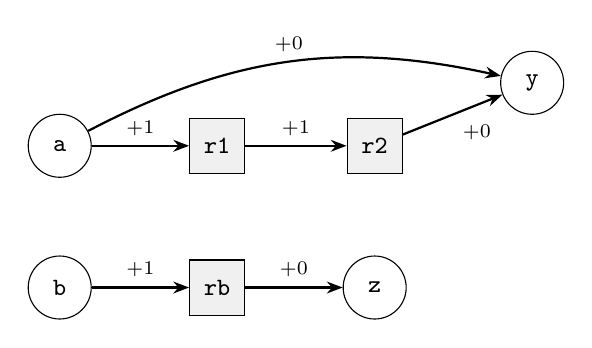
\begin{tikzpicture}[
  sig/.style={draw,circle,minimum size=8mm,font=\small\ttfamily},
  reg/.style={draw,minimum size=7mm,font=\small\ttfamily,fill=black!6},
  arr/.style={-{Stealth[length=2mm]},thick}]
\node[sig] (a) at (0,0) {a};
\node[reg] (r1) at (2,0) {r1};
\node[reg] (r2) at (4,0) {r2};
\node[sig] (y) at (6,0.8) {y};
\node[sig] (b) at (0,-1.8) {b};
\node[reg] (rb) at (2,-1.8) {rb};
\node[sig] (z) at (4,-1.8) {z};
\draw[arr] (a) -- node[above,font=\scriptsize]{+1} (r1);
\draw[arr] (r1) -- node[above,font=\scriptsize]{+1} (r2);
\draw[arr] (r2) -- node[below right,font=\scriptsize]{+0} (y);
\draw[arr] (a) to[bend left=20] node[above,font=\scriptsize]{+0} (y);
\draw[arr] (b) -- node[above,font=\scriptsize]{+1} (rb);
\draw[arr] (rb) -- node[above,font=\scriptsize]{+0} (z);
\end{tikzpicture}
\caption{The \texttt{multipath} fixture. Edges carry their register delays; the cone of \texttt{y} contains \texttt{a} at depths 0 and 2, \texttt{r1} at depth 1 and \texttt{r2} at depth 0. \texttt{b} cannot influence \texttt{y}.}
\label{fig:multipath}
\end{figure}

\subsection{Rank mode (H6, D-014)}
For a mined assertion \code|G(antecedent -> consequent)|, let the \emph{leaves} be its atomic propositions, and $\mathit{off}(\ell)$ the cycle at which leaf $\ell$ is evaluated, relative to the start of the antecedent; $\mathit{off}$ is unknown under \code|until|, \code|F|, \code|R|, repetitions and ranges. Let $A$ be the antecedent leaves with variables, $C$ the consequent leaves, and $\mathrm{cone}(c)$ the sources of signal $c$ with their depths. Then
\begin{align*}
\mathtt{coiFrac} &= \frac{|\{\ell \in A : \forall v \in \mathit{vars}(\ell).\ \exists q\in C,\, c \in \mathit{vars}(q).\ v \in \mathrm{cone}(c)\}|}{|A|},\\
\mathtt{coiDepthFit} &= \frac{|\{\ell \in A : \forall v \in \mathit{vars}(\ell).\ \exists q\in C,\, c \in \mathit{vars}(q).\ \mathit{off}(q)-\mathit{off}(\ell) \in \mathrm{depths}(v, c)\}|}{|A|},
\end{align*}
where a saturated source also fits at any distance above \code|max_depth|, and an unknown offset falls back to cone membership. With no antecedent leaves (an invariant), both are 1. \code|coiUnknown| counts the antecedent leaves with a variable the file does not know; they count as in the cone and fitting: never penalised, but counted.

Offsets depend on the implication: with \code!|->! the consequent starts at the end of the antecedent, with \code!|=>! a cycle later, with \code|->| together with the antecedent. Getting \code|->| right needed a fix (F6 of \ms{H8}): the first version anchored it at the end, as for \code!|->!.

These variables can be used in any \code|<sort>| or \code|<filter>|, e.g. \code|<sort name="fit" exp="coiDepthFit"/>|. On \texttt{multipath} with templates \code|G(P0 -> P1)|, \code|G(P0 -> X P1)| and \code|G(P0 -> X X P1)|, the seven assertions that hold score as derived by hand from the RTL; \code|G(z -> rb)| holds on the trace but \code|z| cannot influence \code|rb|:

% example
\begin{lstlisting}
$ harm --vcd tests/input/coi/multipath/trace.vcd --clk clk --vcd-ss tb::dut \
    --conf tests/input/h6/multipath_rank.xml --dont-print-ass \
    --dump-assertion-info $OUT/rank.json > /dev/null
$ python3 -c "import json; [print(a['text'], a['metrics']['coiFrac'], a['metrics']['coiDepthFit']) for a in json.load(open('$OUT/rank.json'))['assertions']]"
G(a -> XXr2) 1.0 1.0
G(b -> Xz) 1.0 1.0
G(rb -> z) 1.0 1.0
G(z -> rb) 0.0 0.0
\end{lstlisting}

Propositions and numerics can also carry a free-text \code|origin| (\code|<prop exp="..." origin="spec"/>|), reported by \opt{dump-assertion-info} and \opt{dump-coi-report}. trivergence marks the propositions that come from the specification this way.

\subsection{Filter mode, signal level (H7, D-017, D-018)}
\code|<coi ... mode="filter"/>| never tries, for a consequent, an antecedent proposition outside its cone. The rule is \code|coiFrac|'s, so that the two modes share one definition: a proposition is in the cone of a consequent if \emph{every} one of its variables is a source of \emph{some} variable of the consequent. Unknown signals count as in the cone; propositions without variables and placeholders shared by antecedent and consequent are kept. Permutations of plain templates that use an out-of-cone proposition are removed before mining, and decision-tree candidates are restricted to the consequent's cone. HARM reports the search space before and after, and \opt{dump-assertion-info} records it.

\paragraph{Not ``rank mode minus out-of-cone assertions'' (D-018).} For plain templates the two are the same. With decision trees, pruning changes what the greedy tree explores, so filter mode can find in-cone assertions that rank mode misses. Its guarantee is the output of rank mode on a configuration from which, for each consequent, the out-of-cone propositions were deleted by hand; that is how it was validated (\cref{sec:validation}).

\subsection{Filter mode with depths (H8, D-007, D-020)}
\code|depth="bounded"| or \code|"exact"| also uses the depths. An antecedent proposition at distance $d$ cycles before a consequent leaf is kept, for each of its known variables $v$, if some consequent variable $c$ gives:
\begin{center}\small
\begin{tabular}{@{}ll@{}}
\toprule
\code|depth| & condition \\
\midrule
\code|any| (default) & $v \in \mathrm{cone}(c)$ (the signal-level filter) \\
\code|bounded| & $0 \le d \le \max \mathrm{depths}(v,c)$, or $v$ saturated and $d \ge 0$ \\
\code|exact| & $d \in \mathrm{depths}(v,c)$, or $v$ saturated and $d > \mathtt{max\_depth}$ \\
\bottomrule
\end{tabular}
\end{center}
\code|exact| is \code|coiDepthFit|'s rule; the metric and the filter share one function, so filter output with \code|exact| has \code|coiDepthFit| = 1. In \cref{fig:multipath}, \code|y| gets \code|a| at depths 0 and 2: \code|G(a -> X y)| ($d=1$) is kept by \code|bounded| and not by \code|exact|; \code|G(a -> X X X y)| ($d=3$) by neither.

\paragraph{Decision trees (D-007).} A decision-tree operator adds items at indices; each index is at a fixed distance from each consequent leaf, independent of how many items the tree adds later:

\begin{center}\small
\begin{tabular}{@{}lll@{}}
\toprule
Implication & antecedent layout & distance of index $i$ to leaf $q$ \\
\midrule
\code!|->! & \code|dM ##N ... ##N d1 ##N d0| (index 0 is the last cycle) & $i\cdot N + \mathit{off}(q)$ \\
\code!|=>! & the same & $i\cdot N + 1 + \mathit{off}(q)$ \\
\code|->| & \code|d0 ##N d1 ... ##N dM| from the start & $\mathit{off}(q) - i\cdot N$ \\
\bottomrule
\end{tabular}
\end{center}
HARM computes this table rather than hard-coding it: it places a marker at each index and runs the same offset function as \code|coiDepthFit|. A unit test checks 12 template shapes against the table, and mined \texttt{counter} assertions were checked by hand. A (candidate, index) pair is tried only if the candidate fits at that distance.

On \texttt{multipath}, \code|exact| keeps 10 of the 147 permutations, and mines the six structural assertions of the rank example, without \code|G(z -> rb)|:

% example
\begin{lstlisting}
$ sed -e 's#mode="rank"#mode="filter" depth="exact"#' -e 's#\.\./coi/#../tests/input/coi/#' \
    tests/input/h6/multipath_rank.xml > $OUT/filter.xml
$ harm --vcd tests/input/coi/multipath/trace.vcd --clk clk --vcd-ss tb::dut \
    --conf $OUT/filter.xml --dont-print-ass --dump-to $OUT/filter.txt
COI filter (context 'default'): permutations 147 -> 10
$ cat $OUT/filter.txt
G(a -> XXr2)
G(rb -> z)
\end{lstlisting}

\subsection{The out-of-cone report (H9, D-022)}
\opt{dump-coi-report} lists, for each consequent proposition, the antecedent propositions and numerics that cannot influence it, with their \code|origin| and the signals outside the cone; propositions HARM cannot decide (unknown signals) are listed apart, never as ``out''. It is computed from the configuration and the cone file, and does not change mining. For trivergence, a proposition with \code|origin="spec"| outside a cone is a disagreement between the specification (``A influences B'') and the RTL (``it cannot'').

% example
\begin{lstlisting}
$ harm --vcd tests/input/coi/multipath/trace.vcd --clk clk --vcd-ss tb::dut \
    --conf tests/input/h6/multipath_rank.xml --dont-print-ass \
    --dump-coi-report $OUT/report.json > /dev/null
$ python3 -c "import json; [print(c['text'], '<-', [o['text'] for o in c['outOfCone']]) for c in json.load(open('$OUT/report.json'))['contexts'][0]['consequents']]"
y <- ['b', 'rb', 'z']
z <- ['a', 'r1', 'r2', 'y']
\end{lstlisting}

\section{\texttt{harm-coi}: cones and predicates from the RTL}\label{sec:harmcoi}
\texttt{harm-coi} (\file{tools/harm-coi/}) is a Python tool that reads SystemVerilog RTL and writes the \texttt{coi.json} of \cref{sec:coi}. It is the only part of v4 that reads the design; HARM itself stays source-agnostic.

\subsection{The front end (H5a, D-006)}
Two front ends were compared on the six hand-written fixtures of \ms{H4} in a spike: the elaborated syntax tree of pyslang~\cite{slang}, with our own dataflow and control-dependency walk, and the JSON netlist of yosys~\cite{yosys} with its slang front end. pyslang reproduced all six fixtures exactly. yosys needed a version newer than the one packaged on macOS, lost struct fields and parameters, and lowered the conditions that predicate harvesting needs. The decision was \textbf{pyslang 12.0.0}, pinned (Python $\ge$ 3.11). yosys stays an optional, signal-level cross-check in the tests.

\subsection{Computing cones (H5, D-019)}
The front end elaborates the design and extracts, for every assignment, the direct dependencies of its target, with their register delays:
\begin{itemize}
\item \textbf{data dependencies} from the right-hand side, and \textbf{control dependencies} from the conditions of \code|if|, \code|case| (selector and items) and \code|?:|;
\item a register assigned in a clocked process has delay 1; combinational logic, continuous assignments and port connections have delay 0;
\item a register not assigned on every path holds its value, so it is a source of itself at delay 1;
\item \textbf{asynchronous controls} (\code|always_ff @(posedge clk or posedge rst)| where the body reads \code|rst|) and registers on the falling edge of the sampling clock have depths 0 and 1;
\item \textbf{blocking temporaries}: a variable local to a process is replaced by its sources; a visible signal assigned once in a process and read later in it is also a source at delay 0. This last rule came from a test that was wrong (H5, F2): the yosys cross-check and the simulation oracle both showed that forcing such a temporary changes the output, so filter mode must not prune \code|G(t -> y)|.
\end{itemize}
\texttt{cone.py} maps the design's signals to the names HARM sees: relative to the VCD scope, with \code|::| between sub-scopes. With \code|--vcd|, the trace decides which signals are visible: a packed struct dumped as one vector is one signal, the union of its fields. The closure up to \code|--max-depth| sums the delays along paths and marks saturation.

\paragraph{Too large, never too small.} A cone that is too small would make filter mode prune real behaviour; one that is too large only prunes less. So where the RTL leaves a doubt, the signal goes to \code|unknown|, which HARM treats as in every cone: latches (including an \code|always_comb| output not assigned on every path, since \code|unique| and \code|priority| are not trusted to make a \code|case| complete), registers on another clock or on both edges, \code|inout| ports, tasks, a driver that slang reports but the walk does not model, and every target whose cone reaches an unknown signal within \code|--max-depth|.

\subsection{RTL predicates (H10, D-023)}\label{sec:predicates}
\code|--predicates| also harvests the RTL's own conditions as HARM propositions, written in HARM's syntax and names, with \code|origin="rtl"|:
\begin{center}\small
\begin{tabular}{@{}P{0.17\textwidth}P{0.42\textwidth}P{0.33\textwidth}@{}}
\toprule
Kind & from & predicate \\
\midrule
condition & \code|if (c)|, \code|c ? x : y| & \code|c|, and each atom of a compound \code|c| \\
case label & \code|case (s) L:| & \code|s == L| \\
enum (FSM) value & a variable of an enum type & \code|v == C| for every value \\
comparison & with a constant side, anywhere & the comparison \\
reset value & the first \code|if| of a clocked process whose branch assigns only constants & \code|reg == value| \\
\bottomrule
\end{tabular}
\end{center}
Constants are written as sized decimal literals of the signal's width (\code|state == 2'd1|); a 1-bit comparison as the signal or its negation. Predicates on invisible signals, on local variables, or on signals wider than HARM's 511-bit limit (finding F-L5, on the AssertLLM2 design \texttt{sha3}) are dropped and counted. \code|--emit-config| writes a ready-to-run HARM configuration: one context with the predicates, \code|<coi ... mode="rank"/>| pointing at the written file, and \opt{generate-config}'s template and sorts. On the \texttt{counter} fixture (a mod-10 counter with enable):

% example
\begin{lstlisting}
$ harm-coi --top counter --files tests/input/coi/counter/rtl/counter.sv \
    --vcd-scope tb::dut --vcd-recursion 0 --vcd tests/input/coi/counter/trace.vcd \
    --predicates --emit-config $OUT/counter.xml -o $OUT/counter_coi.json
$ grep -E 'prop|coi' $OUT/counter.xml
<prop exp="cnt == 4'd0" loc="a, c, dt" origin="rtl"/>
<prop exp="cnt == 4'd9" loc="a, c, dt" origin="rtl"/>
<prop exp="en" loc="a, c, dt" origin="rtl"/>
<prop exp="rst" loc="a, c, dt" origin="rtl"/>
<coi file="counter_coi.json" mode="rank"/>
$ harm --vcd tests/input/coi/counter/trace.vcd --clk clk --vcd-ss tb::dut --vcd-r 0 \
    --conf $OUT/counter.xml --max-ass 3 --sva --dont-print-ass --dump-to $OUT/counter.txt > /dev/null
$ cat $OUT/counter.txt
always (cnt == 4'b1001 ##1 !(cnt == 4'b1001) |-> cnt == 4'b0)
always (cnt == 4'b1001 && en ##1 1'b1 |-> cnt == 4'b0)
always (rst ##1 1'b1 |-> cnt == 4'b0)
\end{lstlisting}
For GoldMine-style mining, the mode is changed to \code|filter|, with \code|depth| as needed.

\section{Determinism and portability}\label{sec:portability}
v4 was developed on macOS (arm64) and checked on Linux (x86\_64, Ubuntu 22.04), with the rule that both pass the same tests and mine the same assertions. Getting there exposed problems in the build, in the test infrastructure, and in HARM itself. Findings on Linux are numbered F-L1 to F-L10, on macOS F-M1 and F-M2.

\subsection{One toolchain (D-010, H0)}
At the start of the plan, HARM aborted on the development Mac even for \opt{help}: Spot was linked against GCC~12's C++ runtime, ANTLR and HARM against GCC~13's, and Boost against Apple's \code|libc++|, because Boost's build tool ignores \code|CC|/\code|CXX|. Before the fix, ctest even reported the example tests as passing while HARM was aborting at load time. Now every script in \file{third_party/} honours \code|CC|/\code|CXX| (Boost through an explicit toolset), records the compiler in \code|.harm_toolchain|, and CMake warns when HARM is configured with another one. On macOS, Homebrew's GCC~13 cannot compile against the newest Command Line Tools SDK, so the scripts use Xcode's SDK unless \code|SDKROOT| is set.

\subsection{Linux (H11b, H11c, H11f)}
\begin{itemize}
\item \textbf{F-L1: HARM did not build on Linux.} Z3's C++ API overloads \code|bv_val| for \code|int|, \code|unsigned|, \code|int64_t| and \code|uint64_t|. On LP64 Linux \code|uint64_t| is \code|unsigned long|, so the \code|unsigned long long| that the Z3 encoding passed matched none exactly; on macOS \code|uint64_t| is \code|unsigned long long|. The encoder now takes \code|uint64_t| (\ms{H11b}).
\item \textbf{F-L2:} the implication test, which enumerates all short traces for hundreds of pairs, took longer than ctest's default timeout on the slower Linux machine; it has a timeout of one hour.
\item \textbf{F-L3:} the test registration asked yosys for \code|help read_slang|, which exits with 0 even when the command does not exist; the probe now runs \code|read_slang| on a one-line module (\ms{H11c}).
\item \textbf{F-L4} and \textbf{F-L5}, found on real designs, are D-028 (\cref{sec:default}) and the 511-bit limit of harvested predicates (\cref{sec:predicates}).
\item \textbf{F-L9: the log files under concurrent writers} (\ms{H11f}). HARM appends warnings and errors to \code|warning.log| and \code|error.log| as one JSON array, by reading the file, removing the last line and appending. On an empty file the line count underflowed (\code|size_t|), and a concurrent writer could empty the file between another's checks. Parallel ctest runs crashed intermittently, in the same tests as the crashes recorded as an open finding in \ms{H6}. Writers now hold a file lock and a mutex for the whole read-modify-write, and an empty file is handled. Eight processes writing 200 warnings each now leave one valid array of 1{,}600 records. Since \ms{H21}, a record is written over the array's closing line instead of rewriting the file, so a message costs the same however long the log is (2{,}000 warnings on a log of 50{,}000 records: 602\,s before, 0.07\,s after).
\end{itemize}

\subsection{The test tools in \texttt{third\_party} (H11d, H11e, H11g)}
The oracles use Verilator, Icarus Verilog and yosys. v4 adds install scripts for pinned versions (Verilator 5.052, Icarus 13.0, yosys 0.69 with \code|read_slang|), and CMake prefers them over the ones on \code|PATH|, treating a Verilator older than 5 or a yosys without \code|read_slang| as missing. Moving to the pinned Verilator found that the fixtures depended on the simulator's version (D-029):
\begin{itemize}
\item \textbf{F-L7:} the fixture testbenches drew their stimulus from \code|$urandom|, whose sequence for a given seed changed between Verilator 5.031 and 5.052, so the committed traces could not be reproduced. The testbenches now use a xorshift generator written in SystemVerilog (\file{tests/input/stim.svh}), and a test checks that Verilator and Icarus produce the same stimulus.
\item \textbf{F-L6:} the replay oracle negated property consequents with \code|!|, which IEEE~1800 does not allow (\code|not| is required); Verilator 5.052 rejects it.
\item \textbf{F-L10:} Verilator 5.052 implements the end-of-simulation failure of a pending \code|s_eventually|, so the replay oracle now mines with \opt{trace-end} \code|sva|. It also never fails \code!a |-> not (s_eventually p)!, so those controls are checked by a monitor validated on hand-labelled traces.
\item \textbf{F-L8:} the influence oracle assumed both traces had the same signals; Verilator 5.052 no longer dumps a loop variable.
\item \textbf{F-M1:} Verilator did not build on macOS, because Homebrew's \code|flex| is keg-only and its \code|FlexLexer.h| is on no include path; the scripts now put the Homebrew formulas' headers on \code|CPATH| (\ms{H11g}).
\end{itemize}
HARM itself did not change in \ms{H11d}, \ms{H11e} or \ms{H11g}.

\subsection{The same assertions on arm64 and x86\_64 (H12, F-M2)}\label{sec:fma}
After all tests passed on both machines, the evaluation's fixture table still differed on two designs: on \texttt{structs}, macOS mined 1{,}800 assertions and Linux 1{,}839, deterministically on each, for any thread count, from byte-identical configurations, and also with Linux built with the Mac's compiler version. Bisecting by build target, with floating-point contraction turned off in one target at a time, located the cause in two functions of the decision-tree search, the scores
\[
\mathit{cov} = 1 - \frac{\mathit{ATCT}}{\mathit{CT}}\Bigl(1 - \frac{\mathit{ATCF}}{\mathit{CF}}\Bigr), \qquad
H = -p\log_2 p - q \log_2 q .
\]
On arm64, GCC contracts \code|a - b*c| into one fused multiply-subtract by default, which skips the rounding of the product; x86\_64 without FMA instructions rounds it. The decision tree sorts candidates by gain and, with a small effort setting, keeps only the best. Among equal or nearly equal scores, the last bit decides which antecedent is kept, and so the tree, and the assertions. Of 19{,}182 coverage scores computed on arm64, 2{,}644 differed in the last bit from the step-by-step rounded value.

v4 compiles everything HARM's CMake builds with \code|-ffp-contract=off|. Linux is unchanged (it never contracted), and macOS now mines Linux's counts: the fixture table is equal on all 46 runs on both machines. Two tests guard it: the scores are compared bit for bit with a reference that rounds every operation, and \texttt{structs} must mine 1{,}839 assertions. A deeper fix, comparing gains with a tolerance and breaking ties by a fixed key, would remove the dependence on rounding altogether, but it changes the mined assertions on every platform; it was not taken (\cref{sec:limits}).

\subsection{Smaller changes}
\begin{itemize}
\item \textbf{\opt{version}} prints \code|HARM <git describe>| (\ms{H11}, D-027), so users and trivergence can tell which build they run.
\item \textbf{Profiling is opt-in} (\ms{H13}): since v2, every GCC build was linked with \code|--profile| without compiling for profiling, so every run, even \opt{version}, wrote a useless 2.6\,MB \code|gmon.out|. \code|-DHARM_PROFILE=ON| now builds a real \code|gprof| profile.
\item \textbf{\opt{check-dump-eval} files} (\ms{H16}, D-030): v3 named each checked assertion's CSV after its text with some characters deleted, so \code|a != b| and \code|a <= b| overwrote each other's file, and a name over 255 bytes stopped HARM. v4 writes \code|<k>_<text>.csv| and an \code|index.json| that maps each file to its exact assertion, and every row has all five columns. A test recomputes every row from the trace and compares it with the file the index names.
\item \textbf{The proposition table} (\ms{H15}, D-031): \opt{dump-prop-table} writes, for every context, each proposition's value at every sampled cycle, with the trace's files and reset segments, so that another miner (the SAT miner of the miner portfolio) can work on HARM's propositions with HARM's semantics, without a VCD reader or an evaluator of its own. Its tests compare every cell with check mode and with a VCD reader written for the test.
\item \textbf{Findings left open by \ms{H15} and \ms{H16}} (\ms{H17}): \code|^|, \code|&|, \code!|! and \code|~| accept a CSV \code|bool| operand as a 1-bit value, as in SystemVerilog, marked as such when HARM types the variables, so that no parse that worked before changes (D-032); a float numeric's excluded values are compared with the values, not with the cycle index; \opt{vcd-dir} and \opt{csv-dir} concatenate the files in path order (D-033), so a multi-trace run numbers its cycles the same way on every machine.
\item \textbf{Operators as in C and SystemVerilog} (\ms{H18}, D-034): an audit of 1{,}154 expressions against Icarus Verilog, cross-checked with IEEE~1800-2017 and C11, found that HARM's \code|!| took a whole numeric comparison (\code|!x == y| read \code|!(x == y)|), that \code|& ^ \|| bound tighter than comparisons, that a Boolean compared with a number was compared as a truth value, and that some printed propositions re-parsed differently (\code|x - (y - k)| printed \code|x - y - k|). The grammar now follows the standard precedence, comparisons are numbers with a 1-bit result, unary \code|-| exists, and the printer uses the same table; expressions that parsed before keep their trees. The audit is now a test.
\item \textbf{Evaluation as in SystemVerilog} (\ms{H19}, D-035): signedness follows SystemVerilog (an operation with an unsigned operand is unsigned, also for C types), widths are context-determined (a comparison computes its arithmetic operands at its own width), decimal literals are 32 bits, shifts and divisions by zero never stop HARM (they stopped or aborted it before), \code|>>| is logical and \code|>>>| arithmetic, and literals print as they re-parse. A second fixture of 2{,}337 expressions, compared with Icarus Verilog under HARM's x/z rule, covers it; it found two Icarus pitfalls (a \code|?:| with an x condition, and \code|$isunknown| on some 2-state sums). After an optimisation of the comparisons, mining takes within 3\,\% of the time it took before (\texttt{bl\_master10k}, \texttt{sobel1k}). The missing operators (\code|%|, \code|**|, reductions) are future work (\ms{H20}).
\item \textbf{The Docker image} (\file{docker/build.sh}) builds a given git reference with Z3, \texttt{harm-coi}, Verilator and Icarus, and runs the fast tests while it builds.
\end{itemize}

\section{Validation}\label{sec:validation}
Tests written together with the code tend to share its assumptions. Every semantic component of v4 was therefore checked against an \emph{independent oracle}: something that computes the expected answer without HARM's code, or that checks HARM's answer with HARM's own evaluator from the other side. \Cref{tab:oracles} lists them; \file{doc/plan/VALIDATION.md} has every run.

\begin{longtable}{@{}P{0.2\textwidth}P{0.44\textwidth}P{0.28\textwidth}@{}}
\caption{The independent oracle of each component.}\label{tab:oracles}\\
\toprule
Component & Oracle & Result \\
\midrule
\endfirsthead
\toprule
Component & Oracle & Result \\
\midrule
\endhead
Proposition semantics (H1) & Icarus Verilog computes, for 1{,}000 random expressions on 32 random 4-valued rows, both the SystemVerilog value and HARM's documented rule & 0 mismatches with the rule; the SystemVerilog gap measured (D-011) \\
x/z rule (H1b) & 23 pinned propositions, their SystemVerilog values checked against IEEE~1800 and with Icarus & differ on 9 of 23, as documented \\
SVA printing (H1, H1d) & Verilator replays HARM's mined assertions on the same trace: each must never fail, and a negated control of each must fail at least once & 0 failures; all controls fire \\
Spot brackets and \code|->| (H1d) & Spot's \texttt{ltlfilt}: the new texts are equivalent to HARM's formulas, the old ones are not & pass \\
End-of-trace semantics (H1c) & a model of IEEE~1800's finite-trace semantics, written from the standard; 297 assertions $\times$ 4{,}680 traces $\times$ 2 modes & 0 disagreements \\
Z3 equivalence (H2) & brute-force enumeration with HARM's evaluator: for 6-bit variables, all $4^6$ four-valued assignments, 960 pairs; for wide variables, 20{,}000 random rows, 640 pairs. Every ``not equivalent'' must come with a counterexample that HARM's evaluator confirms & 0 unsound; every equivalent 6-bit pair proved \\
Implication (H3) & every Boolean trace of 3 atoms up to length 6, judged by HARM's evaluator: a claimed $A \Rightarrow B$ is refuted if $B$ fails where $A$ does not; 310 generated pairs and 200 pairs in mined shapes, in both end-of-trace modes & 0 unsound (after the D-004 amendment) \\
Atom premises (H3b) & 2{,}000 random traces per pair in which the variables take \code|x|/\code|z| bits; the facts re-checked by enumerating 4{,}096 values & 0 unsound; 10 of 10 facts agree \\
Cone fixtures (H4) & simulation: toggling a signal claimed \emph{outside} a target's cone, with the stimulus otherwise fixed, never changes the target; depths observed with one-cycle pulses & 0 violations in 120 pairs; 102 of 105 depths observed (3 structurally unexcitable) \\
\texttt{harm-coi} (H5) & the hand-written fixtures; the simulation check above on its output; yosys bit-level reachability as a cross-check & exact on 6 fixtures; 0 unsound on 7 designs \\
Rank metrics (H6) & values computed by hand from D-014 on cones validated by simulation & pass, 24 assertions \\
Filter mode (H7) & per-consequent oracle: the union of rank runs on configurations restricted, in Python, to each consequent's cone & equal on 5 fixtures \\
Depth filter (H8) & the D-020 rule recomputed in Python from the printed text; soundness of every kept assertion; the D-007 table counted by hand & pass, 6 designs $\times$ 2 modes \\
Out-of-cone report (H9) & hand-written reports, and the rule recomputed in Python & pass \\
Predicates (H10) & hand-labelled predicates per fixture; Z3 finds no duplicates; no predicate is constant on its trace & pass, 26 predicates \\
Vector indices (H11c) & Verilator prints 14 selects on four vectors every cycle; HARM evaluates the same selects & equal on all $41\times14$ \\
Same results on two platforms (H12) & the fixture table (46 runs) on macOS and Linux, compared count by count & 46 of 46 equal \\
\bottomrule
\end{longtable}

\subsection{Testing the oracles}
An oracle that cannot fail proves nothing. For the components where it was possible, bugs were planted in the implementation, one at a time, and each oracle was run against them (\cref{tab:mutation}). The mutation tests found real gaps, which were closed before the milestones were approved:
\begin{itemize}
\item in \ms{H7}, ``\emph{any} variable in the cone'' instead of ``\emph{every} variable'' passed every fixture, because all fixture propositions had one variable. Two multi-variable propositions were added to each configuration;
\item in \ms{H8}, two planted bugs were caught only by unit tests, because no fixture had a plain \code!|=>! template or a distance beyond \code|max_depth|, and one end-to-end check compared HARM with its own metric. The fixtures gained two templates, and the check a Python rule;
\item in \ms{H5}, each family of oracles missed some bug the others caught: simulation and yosys cannot see depths or self-dependencies, and the fixtures cannot see constructs they do not contain. Only the constructs test caught all six.
\end{itemize}

\begin{table}[t]
\centering\small
\caption{Mutation tests of the oracles: bugs planted in the implementation, and the tests that caught them.}\label{tab:mutation}
\begin{tabular}{@{}lP{0.42\textwidth}P{0.3\textwidth}@{}}
\toprule
Milestone & Planted bug & Caught by \\
\midrule
H3b & facts proved without \code|x|/\code|z| & the hand-labelled facts \\
H3b & premises given to Spot but not to the finite model & the hand-labelled pairs, the command-line test \\
H3b & $p \rightarrow q$ stored as $q \rightarrow p$ & the trace oracle (6 unsound claims) \\
H5 & no control dependencies & fixtures, simulation, yosys \\
H5 & register delay 0 instead of 1 & fixtures (all 6) \\
H7 & decision-tree candidates not pruned & 4 of 5 fixtures \\
H8 & distance off by one & unit tests and 12 end-to-end checks \\
H8 & the tree's index ignored & 11 end-to-end checks \\
H9 & unknown variables counted as out & the unknown-signal fixture \\
H10 & literal width + 1 & 4 fixtures, unit tests \\
\bottomrule
\end{tabular}
\end{table}

\subsection{Tests that were wrong}
Writing tests first means some expectations turn out wrong. They were changed only with a recorded reason, and none to make an implementation pass. Examples: \ms{H5}'s blocking-temporary expectation (\cref{sec:harmcoi}); an \ms{H1} expectation that encoded the SVA precedence bug (\code|s_eventually b_1 until b_2| for \code|F b_1 W b_2|); an \ms{H1c} hand label (\code|!(b W c)| is a strong until, not safety); an \ms{H6} expected order with two equal scores in the wrong order (\code|X| sorts before \code|r| in ASCII, which is the D-001 tie-break).

\subsection{The test suite}
v3 had 35 tests; v4 has 233, run by \code|ctest| in about 32 minutes on either machine. They include the frozen regression baselines of every example (\ms{H0}), the determinism checks, the unit tests, the oracles above, and the documentation checks of this report (\ms{H14}). Tests that need a tool (Verilator, Icarus, yosys, \texttt{harm-coi}'s Python) are registered only when it is found.

\subsection{Not validated}
\begin{itemize}
\item The planned cross-check of the reduction against USM-T's own evaluator was not run: USM-T builds only on Linux, and it would cover only the Boolean and integer subset that the hand labels already cover.
\item No commercial simulator was available to check \code|s_eventually| and \code|not nexttime| at the end of a simulation; the oracle is the standard's semantics.
\end{itemize}

\section{Limitations and future work}\label{sec:limits}

\paragraph{Known limitations.}
\begin{itemize}
\item \textbf{Unknown values.} On cycles where a signal has \code|x| or \code|z| bits, HARM's verdicts can differ from a simulator's (\cref{sec:xz}). An option with SystemVerilog's semantics was withdrawn (D-024): it would break the complementarity of a proposition and its negation that the decision trees and the reductions rely on.
\item \textbf{Reduction cost.} \opt{reduce} \code|implies| and \opt{atom-premises} grow with the square of the number of assertions. On outputs of a few thousand assertions they can take tens of minutes.
\item \textbf{Ties in the decision tree} are decided by the last bit of a floating-point score. Platforms agree because they now round the same operations the same way (\cref{sec:fma}); a different \code|libm| could still change a choice under the entropy heuristic. Rounding-independent tie-breaking would change every platform's results, and was left for a later decision.
\item \textbf{Cones are signal-level.} A write to one bit of a register makes the whole register depend on itself; the schema reserves a per-bit field that is not used. The out-of-cone report does not use depths.
\item \textbf{Mining on real designs.} On the AssertLLM2 designs used in the evaluation, the decision-tree template that \opt{generate-config} writes, over every signal, timed out within 10 minutes on every design tried, so the evaluation there ran only the configurations built from the RTL's predicates (\texttt{harm-coi} \code|--emit-config|), which have far fewer propositions.
\item \textbf{Older limits, unchanged.} Some formulas the grammar accepts cannot be evaluated (\code|F X X (a W c)|, for which Spot gives a non-deterministic automaton); a trace signal named like an operator (\code|W|) cannot be loaded; the \texttt{camellia} example's configuration is not valid XML.
\end{itemize}

\paragraph{The evaluation and the release.} The measurements of what each configuration does on the fixtures, the examples and ten AssertLLM2 designs (D-026) are in \file{eval/results/} and are not part of this report. The release itself, merging \texttt{dev} into \texttt{main} with the tag \texttt{v4} (D-027), is deferred until the maintainers decide; until then, all fixes stay on \texttt{dev} (D-012).

\paragraph{Future work.}
\begin{itemize}
\item the SystemVerilog operators HARM does not read yet: \code|%|, \code|**|, the reductions (\code|&v|, \code+|v+, \ldots) and \code|~^| (\ms{H20}, planned in \file{doc/plan/H20_PLAN.md}), and the functions \code|$onehot|, \code|$countones| and \code|$isunknown|;
\item a faster implication reduction for large outputs;
\item depths in the out-of-cone report (``in the cone, but not at the specification's delay'');
\item a comparison with GoldMine on the designs it supports;
\item diversity-aware selection under \opt{max-ass}, using USM-T's syntactic similarity;
\item a shared core library for HARM and USM-T, so that the two do not drift further apart.
\end{itemize}


\appendix
\section{Reference}\label{sec:reference}

\subsection{New command-line options}
No v3 option was removed or renamed. The new ones, all opt-in:

\begin{longtable}{@{}P{0.3\textwidth}P{0.62\textwidth}@{}}
\toprule
Option & Effect (section) \\
\midrule
\endhead
\opt{reduce} \code+syntactic|equiv|implies+ & redundancy reduction; \code|syntactic| is v3's filter (\cref{sec:reduction}) \\
\opt{keep} \code+stronger|weaker|ranked+ & with \code|implies|: which side of an implication is kept (\cref{sec:implies}) \\
\opt{atom-premises} & with \code|implies|: facts between comparisons, proved with Z3 (\cref{sec:premises}) \\
\opt{atom-premises-max} \code|<N>| & at most $N$ Z3 queries for those facts (default 2{,}000) \\
\opt{dump-implications} \code|<file>| & the dropped assertions and what implies them, as JSON \\
\opt{dump-assertion-info} \code|<file>| & every kept assertion: metrics, leaves, cycle offsets, variables, origins, as JSON \\
\opt{dump-coi-report} \code|<file>| & the out-of-cone report (\cref{sec:coi}) \\
\opt{dump-prop-table} \code|<file>| & every proposition's value at every cycle, as JSON (\code|prop-table| v1, D-031) \\
\opt{trace-end} \code+harm|sva+ & the end-of-trace semantics (\cref{sec:traceend}) \\
\opt{skip-invalid-props} & skip a proposition that does not parse, with a warning \\
\opt{version} & print \code|HARM <git describe>| and exit \\
\bottomrule
\end{longtable}

\subsection{New configuration elements and metric variables}
\begin{longtable}{@{}P{0.38\textwidth}P{0.54\textwidth}@{}}
\toprule
Element or attribute & Meaning \\
\midrule
\endhead
\code|<coi file="..." mode="rank"/>| & a cone file for the context; \code|mode| is \code|rank| (default) or \code|filter| \\
\code|<coi ... mode="filter" depth="exact"/>| & \code|depth| is \code|any| (default), \code|bounded| or \code|exact|; only with \code|filter| \\
\code|<prop ... origin="spec"/>|, \code|<numeric ... origin="..."/>| & free-text provenance, reported in the JSON dumps \\
\code|coiFrac|, \code|coiDepthFit|, \code|coiUnknown| & metric variables, available with a \code|<coi>| (D-014) \\
\code|G(P0)| & invariant templates, without an implication \\
\bottomrule
\end{longtable}
The file format of \code|<coi>| is \file{doc/schemas/coi.v1.json}; the formats of the JSON dumps carry a \code|"version": "1"| field.

\subsection{Decisions}
Every decision of the plan, in \file{doc/plan/DECISIONS.md} unless noted.
\begin{longtable}{@{}lP{0.62\textwidth}l@{}}
\caption{The decisions.}\label{tab:decisions}\\
\toprule
ID & Decision & Milestone \\
\midrule
\endfirsthead
\toprule
ID & Decision & Milestone \\
\midrule
\endhead
D-001 & deterministic output: ranking ties broken by text, ordered collection & H0 \\
D-002 & SVA printing: \code|1'b1|, \code+|=>+, \code|##n|, \code|s_eventually|, \code|.| & H1 \\
D-003 & Z3 equivalence encodes HARM's 4-valued evaluator exactly & H2 \\
D-004 & implication only between safety assertions, in both infinite-word and HARM's finite-trace semantics (amended) & H3 \\
D-005 & COI depth = register crossings, sampled before the rising edge & H4 \\
D-006 & \texttt{harm-coi}'s front end is pyslang & H5 \\
D-007 & decision-tree index $\to$ cycle distance to the consequent & H8 \\
D-008 & by default the stronger assertion of an implication is kept & H3 \\
D-009 & Z3 is optional (\code|HARM_WITH_Z3|, default on) (\file{doc/plan/PLAN.md}) & H2 \\
D-010 & one C++ toolchain for HARM and every library & H0 \\
D-011 & x/z semantics of propositions: HARM's rule, documented & H1, H1b \\
D-012 & fixes stay on \texttt{dev} until the release & --- \\
D-013 & COI sources and targets: visible signals, clock never a source & H4 \\
D-014 & the COI rank metrics & H6 \\
D-015 & mining keeps HARM's end-of-trace semantics; reduction requires both semantics & H3, H1c \\
D-016 & \opt{trace-end} \code|sva|, the neutral view, as an option & H1c \\
D-017 & ``in the cone'': every variable of the proposition & H7 \\
D-018 & COI metrics in filter mode; filter is not rank minus out-of-cone & H7 \\
D-019 & \texttt{harm-coi} conventions: too large, never too small & H5 \\
D-020 & depth modes of the filter & H8 \\
D-021 & SVA printing of \code|->|; brackets in Spot LTL & H1d \\
D-022 & the out-of-cone report & H9 \\
D-023 & RTL predicate harvesting & H10 \\
D-024 & an SVA-semantics option for x/z: withdrawn (\file{doc/plan/H1b_PLAN.md}) & H1b \\
D-025 & atom-implication premises & H3b \\
D-026 & the evaluation's configurations C0--C7 (\file{doc/plan/H11_PLAN.md}) & H11 \\
D-027 & the release: tag \texttt{v4}, \opt{version}, Docker (\file{doc/plan/H11_PLAN.md}) & H11 \\
D-028 & vector indexing follows SystemVerilog & H11c \\
D-029 & fixtures and oracles independent of the Verilator version & H11e \\
D-030 & \opt{check-dump-eval} file names and \code|index.json| & H16 \\
D-031 & the proposition table, \code|prop-table| v1 & H15 \\
D-032 & bitwise operators on \code|bool| operands & H17 \\
D-033 & trace directories in path order & H17 \\
D-034 & operators bind and convert as in C and SystemVerilog & H18 \\
D-035 & evaluation and conversions as in SystemVerilog & H19 \\
\bottomrule
\end{longtable}

\subsection{Milestones and findings}
\begin{longtable}{@{}lP{0.52\textwidth}P{0.3\textwidth}@{}}
\caption{The milestones from v3 to v4, with the findings fixed in each.}\label{tab:milestones}\\
\toprule
ID & Milestone & Findings fixed \\
\midrule
\endfirsthead
\toprule
ID & Milestone & Findings fixed \\
\midrule
\endhead
H0 & regression baselines; deterministic output & --- \\
H1 & proposition and SVA language & F9, F10 (H1's own) \\
H1b & x/z semantics, documented & --- \\
H1c & end-of-trace strength, \opt{trace-end} & SVA precedence \\
H1d & SVA \code|->| and Spot brackets & F7, F8 (found in H8) \\
H2 & Z3 back end, \opt{reduce} \code|equiv| & --- \\
H3 & \opt{reduce} \code|implies| & reduction time on deep assertions \\
H3b & atom-implication premises & --- \\
H4 & \code|coi.json| contract and RTL fixtures & --- \\
H5 & \texttt{harm-coi} & --- \\
H6 & COI rank mode, \code|origin| & --- \\
H7 & COI filter mode & template with too few propositions hung \\
H8 & depth-aware filter & \code|->| offsets (F6) \\
H9 & out-of-cone report & --- \\
H10 & RTL predicates, \code|--emit-config| & --- \\
H11 & evaluation, documentation, \opt{version}, Docker & --- \\
H11b & HARM builds on Linux & F-L1, F-L2 \\
H11c & yosys probe, vector ranges, wide predicates & F-L3, F-L4, F-L5 \\
H11d & Verilator, Icarus and yosys in \file{third_party/} & --- \\
H11e & fixtures and oracles independent of the Verilator version & F-L6, F-L7, F-L8, F-L10 \\
H11f & log files under concurrent writers & F-L9 \\
H11g & \code|install_verilator.sh| on macOS & F-M1 \\
H12 & the same assertions on macOS and Linux & F-M2 \\
H13 & profiling opt-in & --- \\
H14 & this documentation and report & --- \\
H15 & the proposition table, \opt{dump-prop-table} & --- \\
H16 & \opt{check-dump-eval} file names & overwrites, exit on long names (trivergence) \\
H17 & bitwise operators on \code|bool|, float exclusions, sorted trace directories & float exclusions by cycle index \\
H18 & operators and printing as in C and SystemVerilog & precedence of \code|!|, \code|& ^ \|| and comparisons; printing that re-parsed differently \\
H19 & evaluation and conversions as in SystemVerilog & shifts and divisions that stopped HARM; C's signedness rules for \code|logic| \\
H20 & (future work) missing operators & --- \\
\bottomrule
\end{longtable}


\bibliographystyle{plain}
\bibliography{refs}

\end{document}
